\subsection{Упражнение 1}

Вернемся к примеру "Соло на барабане", применим фильтр НЧ до выборки, а затем, опять с помощью фильтра НЧ, удалим спектральные копии, вызванные выборкой. Результат должен быть идентицент отфильтрованному сигналу.

\begin{lstlisting}[language=Python]
if not os.path.exists('263868__kevcio__amen-break-a-160-bpm.wav'):
    !wget https://github.com/AllenDowney/ThinkDSP/raw/master/code/263868__kevcio__amen-break-a-160-bpm.wav
    
from thinkdsp import read_wave

wave = read_wave('263868__kevcio__amen-break-a-160-bpm.wav')
wave.plot()
\end{lstlisting}

\begin{figure}[H]
	\begin{center}
		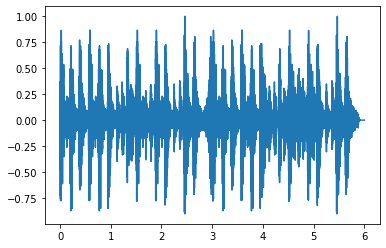
\includegraphics[scale=1]{fig/lab11/lab11_01.png}
		\caption{График сигнала игры на барабанах}
	\end{center}
\end{figure}

\begin{lstlisting}[language=Python]
wave.framerate

44100
\end{lstlisting}

Видно, что сигнал дискретизируется с частотой 44100 hz

\begin{lstlisting}[language=Python]
spectrum = wave.make_spectrum(full=True)
spectrum.plot()
\end{lstlisting}

\begin{figure}[H]
	\begin{center}
		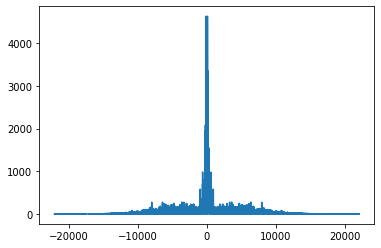
\includegraphics[scale=1]{fig/lab11/lab11_02.png}
		\caption{Спектр сигнала}
	\end{center}
\end{figure}

Применим фильтр НЧ

\begin{lstlisting}[language=Python]
factor = 3
framerate = wave.framerate / factor
cutoff = framerate / 2 - 1
\end{lstlisting}

Применим фильтр сглаживания для удаления частот выше новой частоты сворачивания, которая равна framerate / 2

\begin{lstlisting}[language=Python]
spectrum.low_pass(cutoff)
spectrum.plot()
\end{lstlisting}

\begin{figure}[H]
	\begin{center}
		\includegraphics[scale=1]{fig/lab11/lab11_11_03.png}
		\caption{Отфильтрованный сигнал}
	\end{center}
\end{figure}

Функция, которая имитирует процесс выборки:

\begin{lstlisting}[language=Python]
from thinkdsp import Wave

def sample(wave, factor):
    ys = np.zeros(len(wave))
    ys[::factor] = wave.ys[::factor]
    return Wave(ys, framerate=wave.framerate) 
    
sampled = sample(filtered, factor)
sampled.make_audio()
\end{lstlisting}

\begin{lstlisting}[language=Python]
sampled_spectrum = sampled.make_spectrum(full=True)
sampled_spectrum.plot()
\end{lstlisting}

\begin{figure}[H]
	\begin{center}
		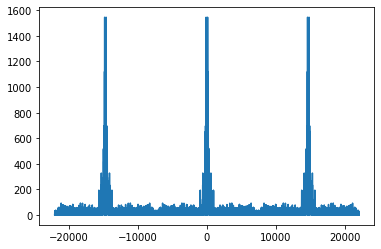
\includegraphics[scale=1]{fig/lab11/lab11_04.png}
		\caption{Получившийся спектр}
	\end{center}
\end{figure}

Видно, что появляются копии спектра

Ещё раз применив фильтр НЧ избавились от них

\begin{lstlisting}[language=Python]
sampled_spectrum.low_pass(cutoff)
sampled_spectrum.plot()
\end{lstlisting}

\begin{figure}[H]
	\begin{center}
		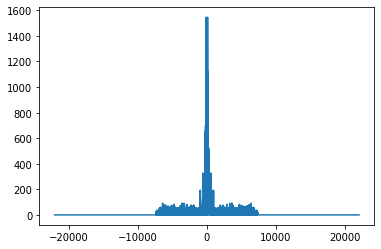
\includegraphics[scale=1]{fig/lab11/lab11_05.png}
		\caption{Результат избавления от копий}
	\end{center}
\end{figure}


\begin{lstlisting}[language=Python]
interpolated = sampled_spectrum.make_wave()
interpolated.make_audio()

spectrum.plot()
sampled_spectrum.plot()
\end{lstlisting}

\begin{figure}[H]
	\begin{center}
		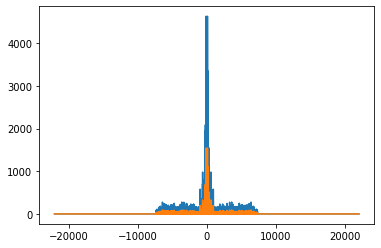
\includegraphics[scale=1]{fig/lab11/lab11_06.png}
		\caption{Сравнение спектров}
	\end{center}
\end{figure}

Увеличим амплитуду в 3 раза

\begin{lstlisting}[language=Python]
sampled_spectrum.scale(factor)
sampled_spectrum.plot()
spectrum.plot()
\end{lstlisting}

\begin{figure}[H]
	\begin{center}
		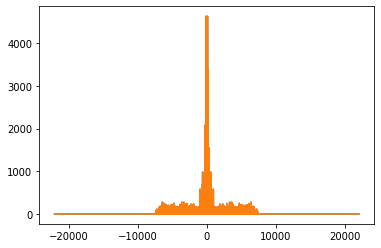
\includegraphics[scale=1]{fig/lab11/lab11_07.png}
		\caption{Сравнение спектров}
	\end{center}
\end{figure}

\begin{lstlisting}[language=Python]
interpolated = sampled_spectrum.make_wave()
interpolated.make_audio()
\end{lstlisting}

Разница едва заметна


\subsection{Вывод}

В данной работе были проверены свойства выборок и прояснены биения и заворот частот.